\documentclass[answers,10pt]{exam}

\usepackage{graphicx}
\usepackage{listings}
\usepackage{amssymb}
\usepackage{float} %figure inside minipage
\usepackage{amsmath} % for maxing matrices easier

\newcommand{\B}[1]{\boldsymbol{#1}}
\newcommand{\R}{\mathbb{R}}
\newcommand{\changes}[1]{{\color{red} #1}}
\lstset{breaklines = true}
\usepackage{xcolor}
\usepackage[english]{babel}
\usepackage{amsmath,amssymb,amsthm,mathdots}
\usepackage{graphicx}
\usepackage[colorinlistoftodos]{todonotes}


\renewcommand{\thequestion}{\arabic{question} }
\renewcommand\questionlabel{\llap{\thequestion)}}


\usepackage{xcolor}
\definecolor{SolutionColor}{rgb}{0.1,0.3,1}

\unframedsolutions
\shadedsolutions
\definecolor{SolutionColor}{rgb}{0.9,0.9,1}
\renewcommand{\solutiontitle}{\textbf{Solution}$:\>$  }




%Mathcal and 
\newcommand{\mb}[1]{\mathbb{#1}}
\newcommand{\mc}[1]{\mathcal{#1}}

%Various possibilities for norms
\newcommand{\norm}[2]{\|#1\|_{#2}}
\newcommand{\normtwo}[1]{\|#1\|_{2}}
\newcommand{\normp}[1]{\|#1\|_{p}}

\newcommand{\rn}{\mathbb{R}^n}
\newcommand{\rnn}{\mathbb{R}^{n\times n}}
\newcommand{\rmn}{\mathbb{R}^{m\times n}}



%Boldface for vectors and tildes
\renewcommand{\vec}[1]{{#1}•}
\newcommand{\mat}[1]{{#1}•}

\newcommand{\vect}[1]{\widetilde{\boldsymbol{#1}}}
\newcommand{\matt}[1]{\widetilde{\boldsymbol{#1}}}

%Column and row equivalence
\newcommand{\roweq}{\stackrel{\text{row}}{\sim}}
\newcommand{\coleq}{\stackrel{\text{col}}{\sim}}

\newtheorem{definition}{Definition}
\newtheorem{example}{Example}
\newtheorem{fact}{Fact}
\newtheorem{remark}{Remark}


%Vector spaces
\newcommand{\rank}{\text{rank}\,}
\renewcommand{\dim}{\text{dim}\,}
\newcommand{\Span}[1]{\text{Span}\,\{#1\}}
\newcommand{\basis}[1]{\left\{ #1\right\}}


%Matrix environments
\newcommand{\bmat}[1]{\begin{bmatrix}#1\end{bmatrix}}
\newcommand{\pmat}[1]{\begin{pmatrix}#1\end{pmatrix}}
\newenvironment{amatrix}[1]{%
  \left(\begin{array}{@{}*{#1}{c}|c@{}}
}{%
  \end{array}\right)
}


%Trace and determinant
\newcommand{\diag}{\mathsf{diag}\,}
\newcommand{\range}{\mathsf{range}\,}
\newcommand{\trace}{\mathsf{trace}\,}


\usepackage{hyperref}
\title{MA 402: Project 4}
\author{Matthew Murray, Johnathan Rhyne}
\date{Fall 2019}
\setlength{\marginparwidth}{2cm}
\begin{document}
\maketitle
\textbf{Instructions}: 


\begin{itemize}
\item Detailed instructions regarding submission are available on the class websitee\footnote{\url{https://github.ncsu.edu/asaibab/ma402_fall_2019/blob/master/projects.md}}.
\item The zip file should contain three files project4.pdf, project4.tex, classnotes.sty. 

\end{itemize}

\vspace{2mm}


\section*{Pen-and-paper exercises}
The problems from this section total $30$ points.
\begin{questions}
\question [10] Let the matrix $\B{A} \in \R^{3\times 2}$ have the SVD 
\[\B{A} = \bmat{ 4 & 0 \\ -5 & -3 \\ 2 & 6} = \frac13\bmat{ 1 & -2 & 2 \\-2 & 1 & 2 \\ 2 & 2 & 1} \bmat{6\sqrt{2}  & 0 \\ 0 & 3\sqrt{2} \\ 0 & 0}  \frac{1}{\sqrt{2}}\bmat{ 1 & 1 \\ -1 & 1}.\]

Let $\B{b} = \bmat{ 1 & 2 & 3 }^\top$. Compute the least squares solution in two different ways:
\begin{parts}
\part Using the normal equation approach;
\begin{solution}
\[ \B{A}^\top = \bmat{4 & -5 & 2 \\ 0 & -3 & 6} \] \\
\[ \B{A}^\top \B{A} = \bmat{4 & -5 & 2 \\ 0 & -3 & 6} \bmat{4 & 0 \\ -5 & -3 \\ 2 & 6} = \bmat{16 & 0 \\ 0 & 0} + \bmat{25 & 15 \\ 15 & 9} + \bmat{4 & 12 \\ 12 & 16} = \bmat{45 & 27 \\ 27 & 45}\] \\
\[ \B{A}^\top \B{b} = \bmat{0 \\ 12} \] \\
\[ \B{A}^\top \B{A} \B{x_*} = \B{A}^\top \B{b} \implies \bmat{45 & 27 \\ 27 & 45} \bmat{x_1 \\ x_2} = \bmat{0 \\ 12} \] \\
Now we look at the 2 equations: \\
$45x_1 + 27x_2 = 0 \quad \And \quad 27x_1 + 45x_2 = 12 $ \\
$45x_1 + 27x_2 = 0 \implies x_1 = \dfrac{-3x_2}{5} \implies 27(\dfrac{-3x_2}{5}) + 45x_2 = 12 \implies x_2 = \dfrac{5}{12} $ \\
$x_2 = \dfrac{5}{12} \implies x_1 = \dfrac{-3 \frac{5}{12}}{5} = \dfrac{-1}{4}$ \\
Therefore, \\
$$
\B{x_*} = \bmat{\dfrac{-1}{4} \\ \\ \dfrac{5}{12}}
$$
\end{solution}
\part Using the SVD of $\B{A}$.
\begin{solution}
\[\B{A}^\dagger = \B{V}_r \B{\Sigma}^{-1}_r \B{U}_r^\top\] \\
\[ \B{V}_r = \dfrac{1}{\sqrt{2}} \bmat{1 & -1 \\ 1 & 1}, \B{\Sigma}^{-1}_r = \dfrac{1}{3\sqrt{2}}\bmat{\dfrac{1}{2} & 0 \\ 0 & 1}, \B{U}_r^\top = \dfrac{1}{3}\bmat{1 & -2 & 2 \\ -2 & 1 & 2}\] \\
\[ \B{V}_r \B{\Sigma}^{-1}_r \B{U}_r^\top = \dfrac{1}{18} \bmat{1 & -1 \\ 1 & 1} \bmat{\frac{1}{2} & 0 \\ 0 & 1} \bmat{1 & -2 & 2 \\ -2 & 1 & 2} = \dfrac{1}{18}\bmat{\frac{1}{2} & -1 \\ \frac{1}{2} & 1}\bmat{1 & -2 & 2 \\ -2 & 1 & 2} \] \\
\[= \dfrac{1}{18}\bmat{\frac{5}{2} & -2 & -1 \\ \frac{-3}{2} & 0 & 3}\] \\
With this solution, we know that $\B{x}_* = \B{A}^\dagger \B{b}$, meaning that $\B{x}_*$ is equal to: \\
$$
\dfrac{1}{18}\bmat{\frac{5}{2} - 4 - 3 \\ \\ \frac{-3}{2} + 0 + 9} = \dfrac{1}{18}\bmat{\frac{-9}{2} \\ \\ \frac{15}{2}} = \bmat{\frac{-1}{4} \\ \\ \frac{5}{12}}
$$

\end{solution}
\end{parts}






\question [10] Consider the line $f(t) = \alpha + \beta t$ that we seek to fit the data 
\[ \mc{D} = \left\{ (t_1,b_1),\dots,(t_n,b_n)\right\}.\]
Assume that $n(\sum_{i=1}^nt_i^2) \neq (\sum_{i=1}^n t_i)^2$. Show that the coefficients $\alpha$ and $\beta$, obtained by solving the least squares problem, satisfy 
\[ \alpha = \frac{(\sum_i t_i^2 ) (\sum_i b_i) - (\sum_it_i)(\sum_i b_i t_i) }{n(\sum_it_i^2) - (\sum_i t_i)^2 }\qquad \beta = \frac{ n (\sum_i b_it_i) - (\sum_i t_i)(\sum_i b_i)}{n(\sum_it_i^2) - (\sum_i t_i)^2 }.\]


\begin{solution}
    note that we can write $\B{A}$, $\B{b}$, $\B{x}$ as: \[\B{A} = \bmat{ 1 & t_1 \\ 1 & t_2 \\ \dots \\ 1 & t_n}\quad \B{b} = \bmat{b_1 \\ b_2 \\ \dots \\ b_n} \quad \B{x} = \bmat{\alpha \\ \beta}\] \\ 
    Now, we have  $\B{A}^{\top}\B{A}$ can be written as \[ \bmat{ \sum{1} & \sum{t_i} \\ \sum{t_1} & \sum{t_i^2}} \] which when multiplied by $\B{x}$ gives us \[ \bmat{\alpha \sum{1} + \beta \sum{t_i} \\ \alpha \sum{t_i} + \beta \sum{t_i^2}} \]
    Now we look at $\B{A}^\top \B{b}$, which when simplified gives us: 
    \[ \bmat{\sum{b_i} \\ \sum{t_i b_i}}  \]
    Next, we solve the 2 equations 
    $\alpha \sum{1} + \beta \sum{t_i} = \sum{b_i}  \text{ and }
    \alpha \sum{t_i} + \beta \sum{t_i^2} = \sum{t_i b_i} $ For $\alpha \text{ and } \beta$, which gives us the 2 following equations: 
    \begin{equation} \label{beta}
        \dfrac{\sum{b_1} - \beta \sum{t_i}}{n} = \alpha = \dfrac{\sum{t_i b_i} - \beta \sum{t_i^2}}{\sum{t_i}}
    \end{equation}
    and 
    \begin{equation} \label{alpha}
        \dfrac{\sum{b_i} - \alpha n}{\sum{t_i}} = \beta = \dfrac{\sum{t_i b_i} - \alpha \sum{t_i}}{\sum{t_i^2}}
    \end{equation}
    
    Now we solve \ref{alpha} for $\alpha$
    \begin{align*}
        \sum{t_i^2}(\sum{b_i} - \alpha n) &= \sum{t_i}(\sum{t_i b_i} - \alpha \sum{t_i}) \\
        \sum{t_i^2} \sum{b_i} -  \alpha n \sum{t_i^2} &= \sum{t_i} \sum{t_i b_i} -  \alpha (\sum{t_i})^2 \\
        \alpha((\sum{t_i})^2 - n\sum{t_i^2}) &= \sum{t_i} \sum{t_i b_i} - \sum{t_i^2} \sum{b_i}
    \end{align*}
    $$
    \alpha = \dfrac{\sum{t_i} \sum{t_i b_i} - \sum{t_i^2} \sum{b_i}}{(\sum{t_i})^2 - n\sum{t_i^2}}
    $$
    or
    $$
    \alpha = \dfrac{\sum{t_i^2} \sum{b_i} - \sum{t_i} \sum{t_i b_i}}{n\sum{t_i^2} - (\sum{t_i})^2}
    $$
    
    Now we solve \ref{beta} for $\beta$
    \begin{align*}
        \sum{t_i}(\sum{b_i} - \beta \sum{t_i}) &= n(\sum{t_i b_i} - \beta \sum{t_i^2}) \\
        \sum{t_i}\sum{b_i} - \beta \sum{t_i} \sum{t_i} &= n\sum{t_i b_i} - \beta n \sum{t_i^2} \\
        \beta n \sum{t_i^2} - \beta \sum{t_i} \sum{t_i} &= n\sum{t_i b_i} - \sum{t_i}\sum{b_i} \\
        \beta(n \sum{t_i^2} - \sum{t_i} \sum{t_i}) &= n\sum{t_i b_i} - \sum{t_i}\sum{b_i}
    \end{align*}
    $$
    \beta = \dfrac{n\sum{b_i t_i} - \sum{t_i}\sum{b_i}}{n \sum{t_i^2} - (\sum{t_i})^2}
    $$
    
\end{solution}


\question [10] Let $\B{A} \in \rmn$ and let $\rank(\B{A}) = n$. Let $\B{x}_*$ be the solution of the least squares problem 
\[ \min_{\B{x}\in \rn}\|\B{Ax}-\B{b}\|_2^2. \]
Define the residual corresponding to the optimal solution $\B{r}_* = \B{b} - \B{Ax}_*$. 
\begin{parts}
\part Starting with the normal equations $\B{A}^\top \B{A x}_* = \B{A}^\top \B{b}$, show that the $\B{x}_*,\B{r}_*$ also satisfy 
\[ \bmat{ \B{I} & \B{A} \\ \B{A}^\top & \B{0}}\bmat{\B{r}_* \\ \B{x}_*} = \bmat{ \B{b}\\ \B{0}}.\]
{\em Remark}: This system is known as the augmented equations and maybe beneficial to use when $\B{A}$ is sparse (i.e., it has many zero entries). 
\begin{solution}
From  $\B{r}_* = \B{b} - \B{Ax}_*$, we get that  $\B{r}_* + \B{Ax}_*= \B{b} = \B{I}\B{r}_* + \B{Ax}_*= \B{b}$. From $\B{r}_* = \B{b} - \B{Ax}_*$,
$$ \implies \B{A}^\top\B{r}_* = \B{A}^\top\B{b} - \B{A}^\top\B{Ax}_*$$
We know that $\B{A}^\top \B{A x}_* = \B{A}^\top \B{b}$
$$ \therefore \B{A}^\top\B{r}_* = \B{0}$$
We can rewrite are results as,
$$\B{I}\B{r}_* + \B{Ax}_*= \B{b}$$
and 
$$\B{A}^\top\B{r}_*+\B{0}\B{x}_* = \B{0}$$
We can combine the results into a matrix as,
\[ \bmat{ \B{I} & \B{A} \\ \B{A}^\top & \B{0}}\bmat{\B{r}_* \\ \B{x}_*} = \bmat{ \B{b}\\ \B{0}}.\]
\end{solution}
\part Show: the vectors $\B{Ax}_*$ and $\B{b}-\B{Ax}_*$ are orthogonal and 
\[ \|\B{b}\|_2^2 = \| \B{b} - \B{Ax}_* \|_2^2 + \|\B{Ax}_*\|_2^2. \]
Provide an interpretation of this result in your words.
\begin{solution}
Compute the dot product between $\B{Ax}_*$ and $\B{b}-\B{Ax}_*$. 
$$\implies (\B{Ax}_*)^\top(\B{b}-\B{Ax}_*)$$
$$= \B{x}_*^\top\B{A}^\top\B{b}-\B{x}_*^\top\B{A}^\top\B{A}\B{x}_*$$
We know that $\B{A}^\top \B{A x}_* = \B{A}^\top \B{b}$
$$= \B{x}_*^\top\B{A}^\top\B{b}-\B{x}_*^\top\B{A}^\top\B{b} = 0.$$
$$\therefore (\B{Ax}_*)^\top(\B{b}-\B{Ax}_*) = 0$$
Also the dot product is commutative,
$$\therefore (\B{b}-\B{Ax}_*)^\top(\B{Ax}_*) = 0$$
We know that $\|\B{Ax}_*\|_2^2 = (\B{Ax}_*)^\top(\B{Ax}_*)$.
$$\therefore \|\B{Ax}_*\|_2^2 = \B{x}_*^\top\B{A}^\top\B{A}\B{x}_* = \B{x}_*^\top\B{A}^\top\B{b}$$
We also know that $\| \B{b} - \B{Ax}_* \|_2^2 = (\B{b}-\B{Ax}_*)^\top(\B{b}-\B{Ax}_*)$ and $\|\B{b}\|_2^2 = \B{b}^\top\B{b}$
$$= \B{b}^\top\B{b} - \B{b}^\top\B{A}\B{x}_* - \B{x}_*^\top\B{A}^\top\B{b}+\B{x}_*^\top\B{A}^\top\B{A}\B{x}_*$$
$$= \|\B{b}\|_2^2 - \B{b}^\top\B{A}\B{x}_* - \B{x}_*^\top\B{A}^\top\B{b} + \B{x}_*^\top\B{A}^\top\B{b}$$
$$\therefore \| \B{b} - \B{Ax}_* \|_2^2  = \|\B{b}\|_2^2 - \B{b}^\top\B{A}\B{x}_*$$
We add the two equations to get,
$$\| \B{b} - \B{Ax}_* \|_2^2 + \|\B{Ax}_*\|_2^2 =  \|\B{b}\|_2^2 - \B{b}^\top\B{A}\B{x}_* +  \B{x}_*^\top\B{A}^\top\B{b}$$
The dot product is commutative, so $ \B{x}_*^\top\B{A}^\top\B{b} - \B{b}^\top\B{A}\B{x}_* = 0$.
$$\therefore \| \B{b} - \B{Ax}_* \|_2^2 + \|\B{Ax}_*\|_2^2 =  \|\B{b}\|_2^2$$
Interpretation: The result is the pythagorean theorem, where the hyppoteneuse is $\|\B{b}\|_2$ and the two legs are $\| \B{b} - \B{Ax}_* \|_2 \text{ and }  \|\B{Ax}_*\|_2.$ 
\end{solution}
\end{parts}




\section*{Numerical exercises}

The problems from this section total $20$ points, and were modified from Boyd and Vandenberghe's ``Introduction to Applied Linear Algebra: Vectors, Matrices, and Least Squares''   Meyer's book ``Matrix Analysis and Applied Linear Algebra.'' MATLAB users may use ``backslash'' for solving the least squares problem, Python users may use \verb|numpy.linalg.lstsq|.  


\question [10] The computer scientist and Intel corporation co-founder Gordon Moore formulated the law that bears his name in a magazine article published in 1965. {\em Moore's law} states that the number of transistors per integrated circuit roughly doubles every 1.5 to 2 years. The table below shows the number of transistors $N$ in 13 microprocessors, and the year of their introduction.

\begin{center}
\begin{tabular}{c|c}
Year & Transistors \\ \hline 
1971 & 2,250\\ 
1972 & 2,500 \\ 
1974 & 5,000\\ 
1978 & 29,000\\ 
1982 & 120,000\\ 
1985 & 275,000\\ 
1989 & 1,180,000\\ 
1993 & 3,100,000\\ 
1997 & 7,500,000\\ 
1999 & 24,000,000\\ 
2000 & 42,000,000\\ 
2002 & 220,000,000\\ 
2003 & 410,000,000\\ 
\end{tabular}
\end{center}
  Based on this law, you hypothesize a model of the form
\[ N \approx \theta_110^{\theta_2(t-1970)},\]
where $t$ is the year and $N$ is the number of transistors.  

\begin{parts}
\part Find the coefficients $\theta_1$ and $\theta_2$ that ``best fit'' the data. {\em Hint}: This is a line fitting problem in disguise. 
\begin{solution}
Define a line fitting problem by taking the common logarithm of both sides of the model:
$$\implies log(N) \approx log(\theta_110^{\theta_2(t-1970)})$$
$$\implies log(N) \approx log(\theta_1) + {\theta_2(t-1970)}$$
We define the following:
$y = log(N)$,
$\alpha = log(\theta_1)$,
$t' = t-1970$,
$\beta = \theta_2$,
and $\B{x} =  \bmat{ \alpha \\ \beta}$.
We solve the line fitting problem by solving the least squares problem shown below. 
$$\min_{\B{x}\in \mathbb{R}^2}\|\B{Ax}-\B{b}\|_2^2$$
$$\B{A} = \bmat{ 1 &0 \\ 1& 2 \\ 1& 4 \\ 1& 8 \\ 1& 12 \\ 1& 15 \\ 1& 19 \\ 1& 23 \\ 1& 27 \\ 1& 29 \\ 1& 30 \\ 1& 32 \\ 1 &33 }$$
and 
$$\B{b} = \bmat{ 2,250 \\ 2,500 \\ 5,000 \\ 29,000 \\ 120,000 \\ 275,000 \\ 1,180,000 \\ 3,100,000 \\ 7,500,000 \\ 24,000,000 \\ 42,000,000 \\ 220,000,000 \\ 410,000,000}$$
\end{solution}
\part Plot the data points (with black crosses) along with the ``best fit'' curve (as a solid red line). A \verb|semilogy| scale is appropriate here.
\begin{solution}
\begin{figure}[H]
    \centering
    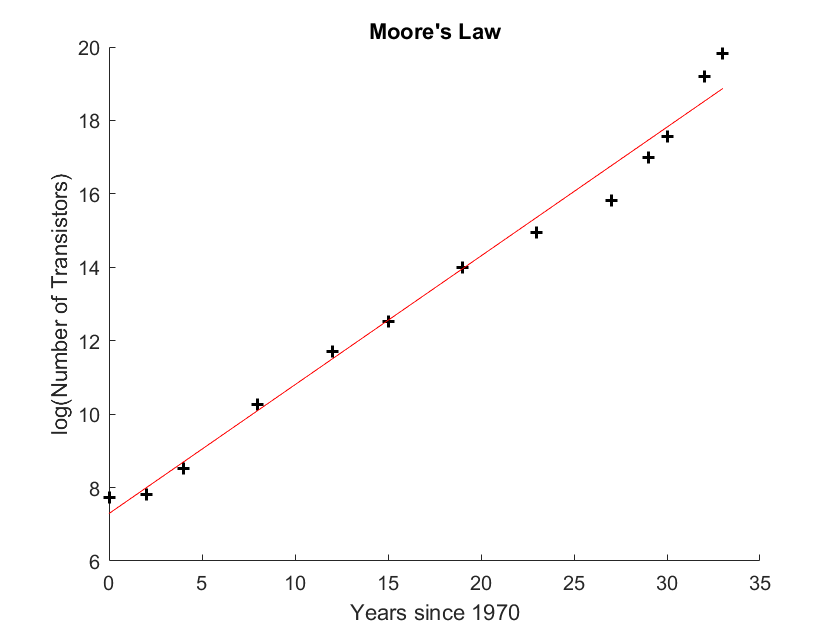
\includegraphics[width=5in]{moorelaw.png} 
    \caption{Number of Transistors over Time} 
    \label{fig:my_label1}
\end{figure}
\end{solution}
\part Use your model to predict the number of transistors in a microprocessor introduced in 2015. Compare the prediction to the IBM Z13 microprocessor, released in 2015, which has around $4 \times 10^9$ transistors.\
\begin{solution}
Our model predicts about $1.2018*10^{23}$ transistors by 2015. This estimate is dramatiocally higher than number of transistors in the IBM Z13 processor. The relative error between the two numbers is nearly zero. 
\end{solution}
\part Comment on whether the data supports Moore's law. 
\begin{solution}
The data here doesn't appear to support Moore's Law. This doesnt mean Moore's Law not valid in the 'bigger' picture.
\end{solution}
\end{parts}



\question [10] Consider the time $(T)$ it takes for a runner to complete a marathon ($26$ miles and $385$ yards). Many factors such as height, weight, age, previous training, etc.\ can influence an athlete's performance, but experience has shown that the following three factors are particularly important:
\begin{center}
\begin{tabular}{ll}
$x_1$ = & Ponderal index  = $\frac{\text{height (in.)}}{[\text{weight (lbs.)}]^{1/3}}$, \\
$x_2$ = & Miles run during  the  previous $8$ weeks,\\ 
$x_3$ = & Age (years).
\end{tabular}
\end{center}
A linear model hypothesizes that the time $T$ (in minutes) is given by $T = \alpha_0 +\alpha_1x_1 +\alpha_2x_2 +\alpha_3x_3 +r$, where $r$ is a residual term that accounts for other factors.
\begin{center}
\begin{tabular}{c|ccc}
$T$ & $x_1$ & $x_2$ & $x_3$ \\ \hline
$181$ &  $13.1$ & $619$ & $23$ \\
$193$ & $13.5$ & $803$ & $42$ \\ 
$212$ & $13.8$ & $207$ & $31$ \\ 
$221$ & $13.1$ & $409$ & $38$ \\
$248$ & $12.5$ & $482$ & $45$
\end{tabular}
\end{center}


\begin{parts}
\part Determine the least squares estimates for the coefficients $\alpha_0,\dots,\alpha_3$ from the available data. 
\begin{solution}
$$
\alpha_0 = 492.0442, \alpha_1 = -23.4355, \alpha_2 = -.0761, \alpha_3 = 1.862
$$
\end{solution}
\part  Estimate the expected marathon time for a 43-year-old runner of height $74$ in., weight $180$ lbs., who has run $450$ miles during the previous eight weeks.
\begin{solution}
The expected marathon time is: 230.7209 mins, which is found by solving: $\alpha_0 + \dfrac{74}{180^\frac{1}{3}} * \alpha_1 + 450 * \alpha_2 + 43 * \alpha_3$
\end{solution}
\part Your instructor (height $68$ in., weight $137$ lbs, and $33$ years old) wants to qualify for the Boston Marathon this year.  How many miles should he run in an eight week period before the marathon to qualify for the Boston marathon? (In his age group, the cutoff for qualification is 3 hours 5 minutes). 
\begin{solution}
We solve: $t = \alpha_0 + x_1 * \alpha_1 + x_2 * \alpha_2 + x_3 * \alpha_3\\$ 

for $x_2$ where we are given the rest of the information, which gives us: $x_2 = 779.8626$ miles
\end{solution}
\end{parts}
For part (c), feel free to use a different person (such as yourself, someone you admire, or a famous mathematician) than the instructor. The qualification times are available at this link: \url{https://www.baa.org/2019-boston-marathon-qualifier-acceptances}.

\begin{solution}
For number 4
$$ $$
For Figure 1
\begin{lstlisting}[language = Matlab]
t = [1970 1972 1974 1978 1982 1985 1989 1993 1997 1999 2000 2002 2003]; %years
T = transpose(t-1970); %time since 1970
n = size(T);
one = ones(n(1),n(2));
A = cat(2,one,T);
b = transpose([2250 2500 5000 29000 120000 275000 1180000 3100000 7500000 24000000 42000000 220000000 410000000]);
y= log(b);
x = (transpose(A)*A)\(transpose(A)*y);
yhat = x(1) + x(2)*T;
scatter(T,y,'k+','LineWidth',1.5)
hold on
plot(T,yhat,'r')
hold off
title("Moore's Law")
xlabel('Years since 1970')
ylabel('log(Number of Transistors)')
y2015 = 10^((x(1))+x(2)*(2015-1970)); %prediction at t-= 2015

\end{lstlisting}
For number 5
\begin{lstlisting}[language = Matlab]
%%
syms A; %Design Matrix
syms T; %Our 'b'
syms a; %matrix of variables
syms AtA;
syms At;
syms RHS; %AtT
syms finalMatrix;
%Setting up our A

A = [1 13.1 619 23;
    1 13.5 803 42;
    1 13.8 207 31;
    1 13.1 409 38;
    1 12.5 482 45];

disp("Rank of A is: " + rank(A)) % gives if 4 which means that A has 
%full column rank meaning AtA is invertible


At = transpose(A);
AtA = At * A;

T = [181;
    193;
    212;
    221;
    248];

RHS = At * T;
a = AtA\RHS; %gives us (AtA)^(-1) * AtT
 %a_0 = 492.0442, a_1 = -23.4355, a_2 = -.0761, a_3 = 1.862
disp("a_0 is: " + a(1));
disp("a_1 is: " + a(2));
disp("a_2 is: " + a(3));
disp("a_3 is: " + a(4));

%% 
%For part b. Height = 74 in. Weight = 180 lbs. MilesRan = 450. Age = 43
x1 = 74/(180)^(1/3);
x2 = 450;
x3 = 43;
t = a(1) + x1 * a(2) + x2 * a(3) + x3 * a(4);
% gives us 230.7209 mins
disp("Estimated time is " + t + " minutes for a person with the given information")
%%
%For part c. Height = 68 in. Weight = 137 lbs. MilesRan = solve for. Age =
%33. Goal is 3 hrs and 5 mins or 185 mins

x1 = 68 /(137)^(1/3);
x3 = 33;
t = 185;

%Now we solve t = a(1) + x1 * a(2) + x2 * a(3) + x3 * a(4) for x2

x2 = (t - a(1) - x1 * a(2) -x3 * a(4)) / (a(3));
% gives us 779.8626 miles
disp("This person will need to run approximately " + x2 + " miles within 8 weeks of the marathon"); 



\end{lstlisting}
\end{solution}
\end{questions}


\end{document}




